\documentclass[nobib]{tufte-handout}
%\geometry{showframe} % for debugging purposes -- displays the margins
\usepackage{amsmath}

% Set up the images/graphics package
\usepackage{graphicx}
\setkeys{Gin}{width=\linewidth,totalheight=\textheight,keepaspectratio}
\graphicspath{{graphics/}}

\title[Psychological Acculturation - Narrative]{Psychological Acculturation: \\
Adjusted Narrative Structure with Notes}
\author[Kreienkamp et al.]{}
\date{March 15, 2021}  % if the \date{} command is left out, the current date will be used

% The following package makes prettier tables.  We're all about the bling!
\usepackage{booktabs}

% The units package provides nice, non-stacked fractions and better spacing for units.
\usepackage{units}

% The fancyvrb package lets us customize the formatting of verbatim environments.  We use a slightly smaller font.
\usepackage{fancyvrb}
\fvset{fontsize=\normalsize}

% Small sections of multiple columns
\usepackage{multicol}

% Provides paragraphs of dummy text
\usepackage{lipsum}

% strike out text
\usepackage[normalem]{ulem}

% APA citations
\bibliographystyle{plain}
\usepackage[style=apa, sortcites=true, sorting=nyt, backend=biber, natbib=true, uniquename=false, uniquelist=false, useprefix=true]{biblatex}
% add reference library file
\addbibresource{references.bib}

% These commands are used to pretty-print LaTeX commands
\newcommand{\doccmd}[1]{\texttt{\textbackslash#1}}% command name -- adds backslash automatically
\newcommand{\docopt}[1]{\ensuremath{\langle}\textrm{\textit{#1}}\ensuremath{\rangle}}% optional command argument
\newcommand{\docarg}[1]{\textrm{\textit{#1}}}% (required) command argument
\newenvironment{docspec}{\begin{quote}\noindent}{\end{quote}}% command specification environment
\newcommand{\docenv}[1]{\textsf{#1}}% environment name
\newcommand{\docpkg}[1]{\texttt{#1}}% package name
\newcommand{\doccls}[1]{\texttt{#1}}% document class name
\newcommand{\docclsopt}[1]{\texttt{#1}}% document class option name

% make question with red triangle
\newcommand\Question[1][2ex]{%
  \renewcommand\stacktype{L}%
  \scaleto{\stackon[1.3pt]{\color{red}$\triangle$}{\tiny\bfseries ?}}{#1}}%
  
% add definition sections
\newtheorem{definition}{Definition}

% framed box section
\usepackage{framed}
\emergencystretch=1em

\begin{document}

\maketitle % this prints the handout title, author, and date

\begin{abstract}
\noindent\marginnote{Abstract: 117 words}One of the key challenges to researching psychological acculturation is an immense heterogeneity in theories and measures. These inconsistencies make it difficult to compare past literature on acculturation, hinder straight-forward measurement selections, and hampers the development of an overarching framework. To structure our understanding of the migration process, we propose to utilize the four basic elements of human experiences (motivations, emotions, thoughts, and behaviors) as a conceptual framework. We use this framework to build a theory-driven literature synthesis and find that the past methodological and empirical literature as well as theoretical models have understudied the more internal aspects of acculturation (motivations and emotions) and have often fallen short of capturing all four aspects of the migration experience.
\end{abstract}

%\printclassoptions

The question of how people change when they get into continuous first-hand contact with other cultures is probably as old as the history of human migration. At the intersection of culture and individual, "psychological acculturation" has taken on a major role within the psychological sciences. Over the past 80 years, researchers have proposed hundreds of models and measurements of acculturation \citep[][]{Rudmin2003a}. Yet, there has been an immense heterogeneity in theories and measures. So, what exactly do we mean when we talk about psychological acculturation? Despite enormous theoretical and applied advances, a conceptual framework allowing for a synthesis of the past literature on psychological acculturation is still missing \citep{Birman2014c}.

\newthought{Problem} This absence of a conceptual framework presents fundamental challenges to researchers, practitioners, and policy-makers in the field. The scattered conceptualization causes issues in the synthesis and development of theories, models, and measurements of psychological acculturation. 

looking at the past, 
\footnote{\textit{"The conceptualization and methods are so variant that it is almost impossible to integrate them, whether intuitively or by some objective procedure such as a formal meta-analysis."} \citep[p. 343]{Taft1981}.}

Some even suggested that psychological acculturation should not be measured until common terminologies and frameworks are available \citep{Escobar2000}.


The immense heterogeneity in theories and measures of psychological acculturation brings researchers, practitioners, and policy-makers to face fundamental challenges when (1) looking back at past literature and interventions, because it becomes hard to compare different effects and outcomes, (2) when looking forward, it becomes hard to choose a definition and measurement for new research and intervention efforts, and (3) more generally, the scattered state of the literature hampers systematic analyses of the literature and the identification of gaps within it.

\begin{figure}[hbt!]
\centering
\caption{Problem Matrix. For thought organization only.}
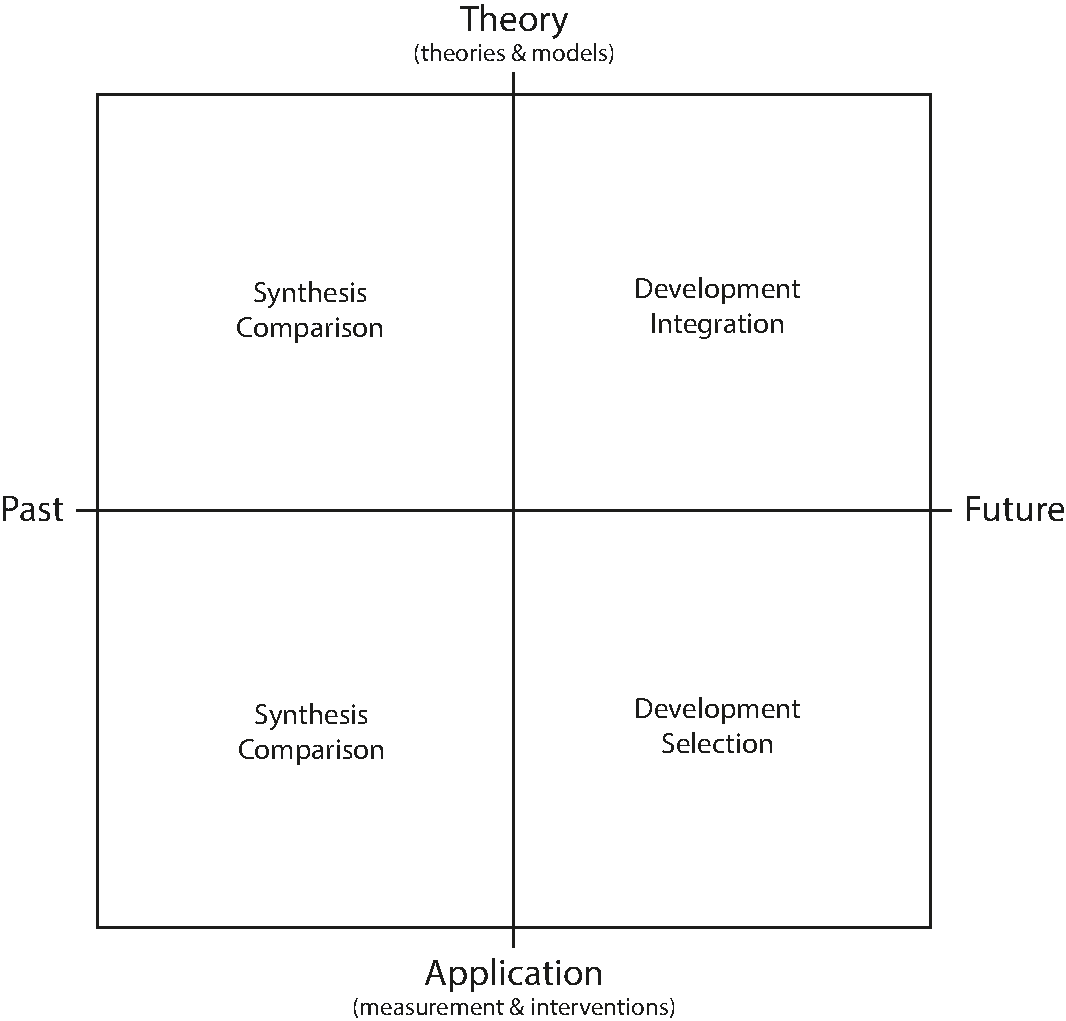
\includegraphics[width=\textwidth]{Figures/ProblemMatrix.pdf}
\label{fig:ProblemMatrix}
\end{figure}


\newthought{Aim} The aim of this paper is, therefore, to offer a descriptive conceptual framework to analyze, measure, and understand the concept of psychological acculturation. Such a framework has a different objective than previous efforts to catalogue literature on cultural adaptation \citep[e.g.,][]{Castels2003}, build multidimensional measures of integration \citep[e.g.,][]{Harder2018}, normative frameworks \citep[e.g.,][]{Ager2008a}, or theories of acculturation \citep[e.g.,][]{Berry2005}. Rather than offering a new measurement, definition, or theory, we aim to build a framework to assess and compare any of these conceptual elements. 
Building on past reviews, we propose to do so by using the basic elements of human experiences and motivation to structure the concept of cultural adaptation.
Once we have introduced our conceptual framework, we will systematically review the past methodological, applied empirical, and theoretical literature on acculturation to apply our framework.

\section{Definition and Focus}\label{sec:definition}\marginnote{I am not sure whether we should have a very extensive discussion of the definitions within the actual paper. And if we do decide to add a definition paragraph, where to put it exactly is another topic. For now I just included it so that we have it to think about.}
Academic discussions of psychological acculturation date back to Plato's cynical discussions of the changes in character when people from different cultures interact (\citeauthor{Plato1926}, ca. 384 B.C.E./1926, Laws 12:949e ff.). The term 'acculturation' was first used within the anthropological literature and likely goes back to the work of \citet{Powell1880}. The most widely reported definition of 'acculturation' is probably the definition by the Social Science Research Council \citep[][p. 149]{Redfield1936}:
\begin{framed}
    \begin{definition}[Acculturation]
        Acculturation comprehends those phenomena which result when groups of individuals having different cultures come into continuous first-hand contact, with subsequent changes in the original culture patterns of either or both groups.
    \end{definition}  
\end{framed}
We would like to remark on three key aspects of this definition. The first remark, is a question of specificity. The main terms used to capture the concept are “phenomena” and “changes”. Following this definition, acculturation therefore is any observable event or fact (i.e., phenomenon) or change that is due to a contact with a new culture. Even as a high-level definition, this lends little guidance as to the structure or the content or the concept. This lends credibility to our aim of finding a framework that structures the aspects of the concept.

The second remark, follows from the previous point, where “phenomena” and “changes” define acculturation both as a process and an outcome at the same time. Although "continuous first-hand contact" lends a stronger weight to the process, phenomena might still relate to outcomes --- as is extremely common in the empirical literature. This lends weight to our focus on assessing process conceptualizations in the literature.

The third remark, concerns the distinction of an individual and a group level. The framing (i.e., "groups of individuals") as well as interpretations of the definition \citep[e.g.,][]{Sam2006b, Berry2005} seem to suggest that acculturation occurs as two related, yet separate, processes of cultural and psychological acculturation. 

In this review we will focus on the individual level and assess aspects of 'psychological acculturation'\footnote{We here also implicitly differentiate 'psychological' from 'individual' acculturation. The \textit{individual} level of acculturation likely includes all aspects of the bio-psycho-social spheres, whereas \textit{psychological} acculturation is presumably limited to the affect, behavior, cognition, desire dimensions.}. For this concept many have used the definition proposed by \citet[][p. 14]{Sam2006b}, based on a research paper by \citet{Graves1967}: 
\begin{framed}
    \begin{definition}[Psychological Acculturation]
        “Psychological acculturation” refers to the changes an individual experiences as a result of being in contact with other cultures, or participating in the acculturation that one’s cultural or ethnic group is undergoing (Graves, 1967).
    \end{definition}
\end{framed}
We again note the group-individual distinction, which in this case seems to have implications for the importance of direct contact. The phrasing of the more passive participation of one's group might relate to research fields of 'indirect contact' \citep[e.g.,][]{Pettigrew2007} and 'imagined contact' \citep[e.g.,][]{Crisp2009}. 

Yet, irrespective of the degree of contact, the main focus of the definition lies on the "individual experiences". This is in direct concordance with our proposal to use the aspects of the human experience to structure the concept of psychological acculturation. 

\section{Conceptual Framework} 

\subsection{Focus Group Discussion}\marginnote{For now I have simply added a summary of the main points we extracted for each acculturation aspect. I assume that if we would like to keep this we will have to shorten this to one or two paragraphs?}
In a first step we reached out to societal stakeholder of the cultural adaptation process to gather information on key adaptation aspects in the lived realities out in the field.

These experience reports formed the foundation of our framework aspects. ...

\paragraph{Methodological Details} Short information section on:\marginnote{Methodological details probably almost entirely into an appendix? (I.e., 1-2 sentences)} \\
participants\\
type of discussion\\
setup (incl., consent, duration, …)\\
coding- and analysis strategy

\paragraph{Behavior} Main points:\\
most visible and often strong expectations\\
focus on social contact (direct and indirect functions) \\
language learning \\
domains important (school, work, sports, music, associations) \\

\paragraph{Cognition} Main points:\\
how we think about ourselves and the world.\\
knowledge (navigational, social, cultural, lingual, norms)\\
identity (break in id, singular ‘refugee' id)\\

\paragraph{Affect} Main points:\\
highlights importance of subjective experience\\
feeling at home and feeling accepted (often conditional on others)\\
feeling useful to society (why job and language are important)\\

\paragraph{Desire} Main points:\\
ABC all instrumental to and embedded in desires\\ \marginnote{This relates well to the concept of 'conation': "the proactive (as opposed to habitual) part of motivation that connects knowledge, affect, drives, desires, and instincts to behavior. Along with affect and cognition, conation is one of the three traditionally identified components of mind." \url{https://dictionary.apa.org/conation}}
need for social interaction (B: contact, A: acceptance)\\
need to be understood and accepted (C: knowledge)\\
need for continuity (C: identity)\\
need for independence (C: language)\\
need for competence and self-esteem (A: useful, purpose)

\subsection{Framework Development}\marginnote{State of Knowledge (?)}
In response to the immense diversity of perspectives within the acculturation literature, Ward and colleagues \citep{Ward2001, Masgoret2006, Ward2019} proposed that the theoretical perspectives commonly found within the literature can be separated into three main traditions\footnote{\citet{Ward2001} mentions six bodies of literature but does not specify further.}. Ward and colleagues have labeled these traditions affect, behavior, and cognition (forming the ABCs of acculturation). Within the affective tradition Ward situates stress and coping literature. \marginnote{I will elaborate on this in the full version.}Behavioral traditions are the cultural learning theories. And social identification theories form the cognitive theories.

\citet{Sam2006b} and others have noted that such a perspective might be useful in structuring the core components of psychological acculturation. We agree and in particular see a broader potential to apply an expanded ABCD structure to the concept of psychological acculturation in general. 

\newthought{Experience}\marginnote{Not sure whether we should discuss 'desires' in more detail. It is a new aspect but might become imbalanced. Maybe wait for the individual sections below.} However, beyond the intuitive appeal of an ABC(D) separation we belief that such a framework also has the potential to offer a theory-driven literature synthesis. A growing body of literature suggests that any human experience can be understood as a set of needs, emotions, cognitions, and behaviors \citep[sometimes referred to as the ABCs or ABCDs of psychology: affect, behavior, cognition, desire; e.g.,][]{Cottam2010, Hogg2005, Jhangiani2014}. \marginnote{It should also be noted that ABC(D) frameworks have been used effectively to structure theories and models across a wide variety of fields --- including research on attitudes \citep{Breckler1984} and ambivalence \citep{VanHarreveld2015}, self-regulation \citep{Ben-Eliyahu2015}, the big five personality traits \citep{Wilt2016}, suicidality \citep{Harris2015} and in clinical interventions \citep{Eifert1989}, and even the review of acculturation literature \citep{Ward2001, Ward2019}. Interestingly, the affect, behavior, and cognition structure has even found application in the development of human-like machines \citep{Guo2020}.}Following the premise that any human experience can be perceived within these four basic elements, we belief that the an ABCD framework of acculturation would not only summarize theoretical traditions within the acculturation literature, but could offer a comprehensive and theory-driven framework to structure and analyze the concept of psychological acculturation.

\newthought{Examples} Psychological acculturation in this framework might, for example, be understood or measured in terms of behavioral acculturation, such as language use, or voting; cognitive acculturation, such as ethnic identification, or cultural values endorsement; affective acculturation, such as feeling at home, or loneliness; motivational acculturation, such as the satisfaction of competence or independence needs; or as a complex combination of any or all of these aspects (also see Table \ref{tab:Examples}1). 

\begin{table}[hbt!]
\caption{Examples for Acculturation Aspect Measures (To be combined with Table 3)}
\label{tab:ExamplesTab} 
\begin{tabular}{@{}llll@{}}
\toprule
Affect              & Behavior                                     & Cognition                          & Desire                \\ \midrule
Lonely              & Language   use                               & Ethnic   identification            & Competence            \\
Feeling at home     & Civic   Participation (voting, ...)          & Cultural   values                  & Independence          \\
Satisfied with life & Performance   (work, ...)                    & Acculturation   orientation        & Self-coherence        \\
Proud               & Media   consumption                          & Preferences   (food, friends, ...) & Belonging             \\
Comfortable         & Education                                    & Knowledge                          & Achievement           \\
Enjoy               & Peer   contacts                              & Importance   ratings               & Justice               \\
At ease             & Food   consumption                           & Inner   thought language           & Growth                \\
Well-being          & Cultural   habits (holidays ...) & Perceived   obligations            & Respect               \\
Worry               & Delinquance                                  & Beliefs                            & Acceptance            \\
Trust               & Marriage                                     & Stereotypes                        & Identity   continuity \\
...                 & ...                                          & ...                                & ...                   \\ \bottomrule
\end{tabular}
\end{table}

\newpage
In the next sections we will look at each of the aspects in more detail.

\newthought{Affect} 
\marginnote{Definitions not necessary for main text. The field of emotional experiences seemed the most difficult to grasp. Everyone has an understanding of what it should mean but I couldn't find anyone providing an actual definition. @Kai: Since you have worked on this before, is there some agreement on terms and models recently?}
\begin{framed}
    \textbf{Definition Struggle:}\\ 
    \begin{quote}
        \begin{itemize}
            \item Affect: "Affect is the collective term for describing \textit{feeling states} like emotions and moods. Affective states may vary in several ways, including their duration, intensity, specificity, pleasantness, and level of arousal, and they have an important role to play in regulating cognition, behavior, and social interactions." \citep[][p. 49]{Niven2013}
            \item Feeling: The subjective experience aspect of an emotional state. That is, the phenomenal experience (i.e., sensation) of affect. Inevitably pleasantness evaluation but can be more complex.
            \item Emotion: Affective state. Many different traditions (e.g., feeling-, motivation-, evaluation traditions, see \citealp{Scarantino2016}). Dimensions: valence (sad vs. happy), arousal (anger vs. sadness), duration (e.g., sadness vs. grief), complexity (e.g., anger vs. hate), consciousness (e.g., fear of spiders vs. fear of failing in life), speed (fear vs. jealousy ~ amount of cognition), motivation (rage vs. sadness ~conation/behavioral activation). Also, sometimes considered a mode of the mind.
            \item Mood: Affective state. Less specific, less intense and less likely to be provoked or instantiated by a particular stimulus or event.
        \end{itemize}
    \end{quote}
\end{framed}

The \textit{affect}\marginnote{definition and link to experience} aspect of the human experience entails the human capacity to feel. These feeling states include emotions and moods and might vary along a variety of dimensions, including valence (positive/negative), arousal (high/low energy), duration (short/long), temporal focus (past/future), or complexity (basic/mixed). Affect has also been well established as one of the key aspects of the human experience \citep{FeldmanBarrett2007}. And while a generally agreed upon model and definition of emotions (the most prominently investigated affective state) is still missing \citep[e.g.,][]{Scarantino2016}, \marginnote{link to culture and cultural differences}there is a growing consensus that emotions are profoundly impacted by cultures \citep[e.g.,][]{Holodynski2012}. While there is some evidence that certain emotions might be universal, evolutionary, and present at birth \citep[e.g.,][]{Ekman1999, FeldmanBarrett2006}, there seems to be converging evidence that some aspects of the emotional experience (e.g., appraisal, expression, regulation, and shared meanings) will always be influenced by culture \citep[][]{Holodynski2012, Matsumoto2012, Kitayama2006}. Some even argue that the entire emotional experience can only be seen as a cultural phenomenon \citep[e.g.,][]{Mesquita2003, Boiger2018}\footnote{is this too vague? Should I add a half sentence on their arguments?}. In sum, previous literature has argued that affect is a fundamental aspect of the human experience and that emotional experiences (or at least their expressions) are different between cultures.

Inversely, emotions are also part of culture. For example, shared emotional experiences are often seen as an important cultural glue \citep{Rensmann2004, Kitayama1994}, emotions are ubiquitous in cultural politics and narratives \citep{Ahmed2014}, and emotions are often fundamental in place attachment and local cultural identities \citep{Smith2016c}. Moreover, for individual cultures, emotions and their expressions often deeply entangled with individual cultural aspects \citep[e.g., see][for a discussion of how different emotions lay at the heart of Chinese cultural elements]{Sundararajan2015}. 

Moreover,\marginnote{Link to inter-group and cultural contact. Not sure whether this paragraph is necessary.} there is also substantial evidence linking emotions structurally to inter-cultural contact. Literature on inter-group contact has for example argued that emotions are important in whether people get into contact with other groups \citep{Esses2002} and that emotions take up a functional role in inter-group processes more generally \citep{Iyer2008}. Also more specific inter-cultural contact literature has highlighted a functional role of emotions in the interactions between cultures \citep[e.g.,][]{Stephan1992}.

Finally,\marginnote{Link to well-being in social change. Not sure whether this paragraph is necessary.} for a perspective of acculturation as an adaptation process, affect is also an important component. As an integral part of the human experience, emotions have long been a gauge of adaptation to social change and major life events \citep[e.g.,][]{Smith1990, Pacella2017}. Phenomena such as culture shock \citep{Ward2001a} and homesickness \citep{VanTilburg1996} are common examples of how social change can have an emotional impact on well-being and might function as an indicator of adaptation. 

From these findings it is not surprising that affect and emotion have also been discussed within the psychological acculturation literature. \citet{Ward2001} in her review of the acculturation traditions, describes the stress and coping literature --- especially Berry's concept of acculturation stress \citep{Berry1997b} --- as the affect component of acculturation. The main concepts that constitute the affective dimension are the psychological and emotional well-being as part of the psychological adaptation process \citep[including, for example life satisfaction and depression][]{Ward2019}. However, beyond the theoretical stress literature tradition, there are also more immediate models and measurements of emotional acculturation. There is, for example, a relatively young tradition of 'emotional acculturation' as a distinct concept, in which acculturation is understood as the similarity in emotional patterns \citep[see][for a review]{DeLeersnyder2017}. But also individual emotions, such as 'feeling accepted' \citep{Jasini2018}, or 'pride' \citep{Suinn1995} have received attentions as discrete aspects of acculturation. 

\newthought{Behavior} 
\begin{framed}
    \textbf{Definition Struggle:}\\ 
    \begin{quote}
        \begin{itemize}
            \item Human behaviors are the activities, actions, or mannerisms of individuals (or groups(?)).
            \item dimensions: conscious vs. subconscious; over vs. covert; voluntary vs. involuntary; towards the self, others, the environment 
        \end{itemize}
    \end{quote}
\end{framed}

The \textit{behavior} aspect of human experiences\marginnote{definition and link to experience} is often the most outward and visible aspect of who we are. Human behaviors --- that is actions and mannerisms --- are also one of the most prominent methods of interactions with the self, the environment, and others. For many, behaviors have been perceived as part of the human experience since early psychological behaviorist movement\footnote{We should probably distinguish psychological behaviorism from methodological, radical, and logical behaviorism. Or we just assume that this is clear. Probably not the most important thing here.} \citep[e.g.,][]{Syngg1949}. While some theories still retain the 'radical behaviorist' essence that behavior is fundamentally a reactive re-enforcement process \citep[largely learning and habit theories; e.g.,][]{Hayes2001}, most psychological accounts of behavior, now consider it an outcome of other experience elements \citep[e.g.,][]{Ajzen2019}. Despite this shift, many theories of human experiences still include behaviors as a key element \citep[e.g.,][]{Breckler1984, VanHarreveld2015, Ben-Eliyahu2015}.

There is also a clear link between behaviors and culture.\marginnote{link to culture and cultural differences} Large parts of the human behavioral repertoire are learned behaviors (i.e., extra-somatic or extra-genetic) and especially social behaviors are often culturally transmitted \citep{Legare2019, Whiting1980}. Cultural differences are, thus, often most visible in behavioral differences, including language use, dress- and food preferences, rituals and habits, as well as behavioral norms more generally \citep[e.g., social norms, as well as formal rules and laws; e.g.,][]{Hofstede2001}. 

Yet, inversely, behavior is also a manifestation of culture in most cultural contexts. One notable example for this has been the literature on cultural change, which has often highlighted that cultures often change through changes in their behavioral norms \citep[e.g.,][]{Varnum2017}. One prominent recognition of this relationship between culture and behavior, has been the protection of indigenous cultural practices as a manifestation of their culture \citep[Art. 11]{UnitedNations2007}. 

Moreover,\marginnote{link to contact. Not sure whether this is relevant. Could be expanded if necessary} behaviors also constitute the most common exchange between cultures. Inter-group interaction behaviors often form the basis for many inter-cultural contacts and exchanges \citep{Maxwell2017, Sam2010}. 

Considering adaptation\marginnote{link to adaptation. Not sure whether this is relevant} as an important definition of acculturation also highlights the relevance of behaviors. Behaviors have, in the past, both been considered as an aspect of adaptation and have been linked to adaptation in terms of well-being. Social skills and behaviors have, for example, been considered as indicators of adaptive behaviors within the field of disability studies \citep[e.g.,][]{HyoJungLee2007}. Additionally, reviews have linked behavior transitions to adaptations in well-being \citep[e.g.,][]{Luhmann2012}. 
In sum, behaviors are a fundamental aspect of the human experience, and while they are often a product of cultural learning they at the same time form physical manifestations cultures. Behaviors also lay at the very foundation of many cultural contacts and can be essential in forming an adaptive relationship with one's environment.

Given the overt nature of behaviors\marginnote{Link to acculturation literature} and their interconnectedness with culture, behaviors have also been a prominent aspect of the acculturation literature. Ward and colleagues \citeyear{Ward2019} in their review have identified cultural learning theories as one key literature tradition that has focused on behavioral aspects of acculturation. They relate these learning theories to the acquisition of effective skills and competences as the behavioral operationalizations \citep[including, verbal and non-verbal communication skills][]{Ward2001}. Other examples of behavioral conceptualizations of acculturation (not mentioned by Ward and colleagues), include civic participation \citep[e.g., voting;][]{Lessard-Phillips2020}, inter-ethnic marriage \citep[e.g.,][]{Song2009}, and media consumption \citep[e.g.,][]{Shoemaker1985}. 

\newthought{Cognition} 
\begin{framed}
    \textbf{Definition Struggle:}\\ 
    \begin{quote}
        \begin{itemize}
            \item thinking, awareness, information processing (also relates to intellectual functioning)
            \item aspects: attention, the formation of knowledge, memory and working memory, judgment and evaluation, reasoning and "computation", problem solving and decision making, comprehension and production of language.
            \item "The mental action or process of acquiring knowledge and understanding through thought, experience, and the senses" \url{https://www.lexico.com/definition/cognition}{Lexico}
            \item "all forms of knowing and awareness, such as perceiving, conceiving, remembering, reasoning, judging, imagining, and problem solving." \url{https://dictionary.apa.org/cognition}{APA Dictionary of Psychology}
        \end{itemize}
    \end{quote}
\end{framed}

The \textit{cognition} aspect of the human experience\marginnote{Definition and link to experience} is concerned with the thinking processes and can include elements such as knowledge, evaluations, decision making, as well as language. Because these processes include conscious awareness and reflection of one's perceptions, cognition is probably the aspect that is linked to experience the clearest \citep{Jacobs1998}. The cognition aspect also has a clear and longstanding relation to culture \marginnote{Link to culture and cultural differences}. Cultural knowledge, values, identities, beliefs, and attitudes are likely the most widely discussed aspects of non-material culture \citep[e.g.,][]{DiMaggio1997}. Yet at the same time cognitions are also substantially influenced by culture \citep[e.g., through social norms][]{Gelfand2011}, which also relates to cultural differences in terms of basic cognitions processes \citep{Nisbett2002}.

Cognitions have also been highlighted\marginnote{Link to inter-group and cultural contact. Not sure whether this is necessary} as functional elements of interactions between cultures. An indirect effect of cognitions are, for example, the cultural affordances of values that structure the contact \citep[e.g.,][]{Ramstead2016}. Beyond the indirect roles of cognitions, thought processes are also a well-established cornerstone of inter-cultural contact perceptions \citep[e.g., out-group attitudes;][]{Stephan2000a}.

Finally,\marginnote{Link to adaptation. Not sure whether this is necessary.} cognitions are also relevant if one considers them in the light of an adaptation process. Processes such as meaning making, self-image restoration, and dissonance reduction have established cognitive adaptation as a vital element in well-being and adaptation processes \citep[e.g.,][]{Czajkowska2017}. In sum, cognitions are a prominent aspect of the human experience, and are intimately intertwined with conceptions and influences of culture. Cognitions also structure and gauge cultural contacts and are a key process of human adaptation.

Given the pertinent connection between culture and cognitive processes,\marginnote{Link to acculturation literature.} it might come as little surprise that cognitions have also played a major role in the acculturation literature. \citet{Ward2001} have identified literature traditions on ethnic identity and group perceptions within the field. Within this cognitive tradition, Ward and colleagues particularly focus on Berry's \citeyear{Berry1997b} acculturation attitudes \citep{Ward2019}. Beyond the cultural attitudes tradition, the acculturation literature has recently also focused on several other cognitive conceptualizations of psychological acculturation, including cultural values \citep[e.g.,]{Marin2003} and stereotypes \citep[e.g.,][]{Stanciu2018}. 

\newthought{Desire} 
\begin{framed}
    \textbf{Definition Struggle:}\\ 
    \begin{quote}
        \begin{itemize}
            \item Motivation is the driving force of the human experience (purpose and direction; reason; the why).
            \item Forms: desires (emotional), goals (cognitive); needs (necessity), wants (would like to have); conscious vs. unconscious; physiological motives and psychological motives; internal (also ~ drives) vs. external; change vs. conservation
            \item conation: "the proactive (as opposed to habitual) part of motivation that connects knowledge, affect, drives, desires, and instincts to behavior." \url{https://dictionary.apa.org/conation}{APA Dictionary of Psychology}
        \end{itemize}
    \end{quote}
\end{framed}

The \textit{desire} aspect \marginnote{Definition and link to experience} encompasses the motivational forces of the human experience. The role of motivation in the phenomenological tradition is particularly interesting because some suggest that it is the motivational aspect that structures and connects the other three aspects of affect, cognition, and behavior \citep[e.g.,][]{Hilgard1980}. As for the different forms of motivation, while many ways of organizing motives have been proposed, one distinction particularly relevant to our discussion is a distinction between the experiences of psychological needs (necessary) and psychological wants \citep[desired without necessity][]{Esposti2015}. There is some evidence that, while some basic human needs are universal and innate \citep[e.g.,][]{Ryan2000}, most wants and some needs might be more socially constructed and thus depend on culture \citep[e.g.,][]{McInerney2016, Morling2017}. One such example might be the case virtuous motivation --- the drive act in a manner that is seen as virtuous in one's society \citep{Stohr2017}.\marginnote{Link to culture and cultural differences} Such a motivation highlights how the motivation is embedded within the culture that defines what a virtue is and likely differs between cultures. Yet at the same time this example also highlights that the concept of culture in parts consists of motivational ideals \citep[or oughts; e.g., see][]{Markus1991}.

Psychological needs\marginnote{Link to inter-group and cultural contact. Maybe unnecessary.} have recently also been highlighted as a key element in inter-group relations \citep{Dovidio2017}. Among other reasons motivation is said to be relevant because need fulfillment is one of the main reasons for engaging in inter-group contacts in the first place \citep{Kitayama2007} and needs might lay at the core of inter-group and intercultural conflicts more specifically \citep{Hassler2021, Shnabel2008a}.

Moreover, motivation is also relevant to adaptation\marginnote{Link to adaptation. Maybe unnecessary} outcomes. Needs have long been linked to different well-being regulations \citep[e.g.,][]{Steverink2006}. And recently first evidence has emerged that shows how motivations might fundamentally drive adaptation processes \citep{Dignath2020}. 
In sum, motivation is one of the most interconnected experience aspect that also has a deep connection to culture, cultural contacts, and psychological adaptation.

Yet, despite these connections,\marginnote{Link to acculturation literature} motivation is seldom discussed as a distinct aspect of the psychological acculturation concept. Few of the past reviews have examined its role within the literature or the concept \citep[including, ][]{Ward2001a, Ward2019}. However, in recent years needs and wants have been discussed more frequently as a conceptual aspect of psychological acculturation --- with more researchers looking at migration driven by reason for migration \citep{Sandu2018}, as well as the motivations of acculturation orientation s\citep{Recker2017a}, acculturation behavior \citep{Reece2000}, and psychological adaptation \citep{Safdar2003}. 

\newthought{Process}
%% Dynamic process rather than static end-product: 
% Experience can answer this call because it can only be understood based on past experiences
A final, fundamental factor we would like to address in the experience framework is the understanding of psychological acculturation as a dynamic process rather than a static end-product. That psychological acculturation is a developmental process, and that ``acculturation occurs when two independent cultural groups come into \textit{continuous first-hand contact over an extended period of time}'' \citep[][186]{Berry1989} seem to be a generally accepted assumption within the field\footnote{also see '\nameref{sec:definition}' section}. Yet, within the empirical literature, few studies have actually considered the theoretical implications of migration as a process and even fewer have methodologically followed the trajectories of migrants over time. Recent years have seen a growing awareness of this discrepancy \citep[e.g.,][]{Brown2011, Ward2019}. We believe that the experience framework of psychological acculturation, as it is presented here, is ideally suited to deal with this conceptualization as a developmental process. Philosophers of the phenomenological tradition have long highlighted that subjective experience can only be understood within the history of past experiences \citep[e.g.,][]{Heidegger1867}. 

\newthought{Experience elements and lived experience}
While we have introduced the four experience aspects as distinct elements it is important to note that both in theory and in practice affect, behavior, cognition, and desire are not experienced as distinct entities. As an example, most emotions have a cognitive component just as most cognitions have an emotional value. Similarly, motivation is commonly conceives as having both emotional (e.g., desire) and cognitive (e.g., goals) aspects, both of which are often directed towards behaviors (i.e., conation). Muddying the waters further is the difficulty that many operationalizations (and empirical measures) of psychological acculturation are complex concepts in themselves. Concepts such as satisfaction or distress, which are common measures of acculturation, famously include emotional and cognitive components. 

Yet, despite the interdependence of aspects and the complexity in the lived experience, the four elements can consistently be identified within experiences and concepts --- they remain qualitatively different aspects of the experience. And as such, they offer a pragmatic lens to structure the psychological acculturation concept \citep{Kuhn1962}. Differentiating the four (needing, feeling, thinking, doing) qualities of an experience in the what we consider psychological acculturation to be, allows us to structure our discussions of past, current, and future theories and measures of psychological acculturation.

\newthought{Features}\footnote{Not an actual heading I think} 
Now that we have introduced the individual experience elements in detail, we would like to speak to the qualities of such a framework more broadly. We belief that utilizing the elements of the human experience to structure the concept of psychological acculturation offers a set of valuable features, which address past conceptual issues. 

Firstly, the experience approach is based on basic human faculties, that is generally speaking every healthy person has the capacity for emotions, thoughts, needs, and behaviors. Focusing on fundamental faculties relevant to any conscious person makes the framework widely applicable across cultural contexts. ABCD frameworks have, for example, been found across cultures \citep[e.g.,][]{Bhawuk2011} and likely structure human forebrain functioning \citep{Swanson2020}\footnote{It is important to note that while anyone will have motives, emotions, thoughts, and behaviors, what one needs (e.g., belongingness or independence), feels (e.g., sadness or happiness), thinks (e.g., identification or disinterest), or does (e.g., studying or working) is highly ideographic. It is this ideographic content that makes the framework relevant to such a broad range of migration contexts. Yet it is the content-free structure --- the presence or absence of the basic elements in conceptualizations of acculturation --- that is transferable across contexts and studies, enabling comparisons and broader conceptual discussion. It should also be noted that in our opinion such a framework does not stand in conflict with cultural or indigenous psychological concerns of an absolutist, or deterministic psychology \citep[e.g.,][]{Kim2006a}. In fact, cultural psychologists, together with many decolonial researchers, have long argued that the individual embedded and lived experience should gain a more central role in our theoretical developments \citep[e.g., ontological turn;][]{Pedersen2020}}.

Secondly, because affect, behavior, cognition, and desire broadly capture the human experience, the experience framework comprehensively captures the psychological element of acculturation. The framework, thus, captures a broad and complex phenomenon while still offering a clear and theory-driven structure of the concept and its applications. 
As such it focuses on how individuals perceive the acculturation process. This also means that non-psychological aspects such as biological, cultural, or societal changes are not captured directly but only to the extent to which they impact the experiences of the involved people. \sout{While sociologists or political scientists might aim to capture the group-level changes more specifically, or medical professionals might want to assess physiological changes due to inter-cultural contact this is not the focus of psychological acculturation.} 

Thirdly, experiences are also relevant across time-scales. In most cases experiences rely on past experience and collectively generate the present experience \citep[also see][]{Husserl1959, Heidegger1867}. As such, experiences are scale-able evaluations --- of a single situation, a recent period, or a life-long journey \citep[e.g.,][]{Clewett2019}. There is usually a clear 'temporality' to human experiences and experiences can focus on the past, present, and even the future.

Finally, the experience conceptualization of psychological acculturation is inherently a bottom-up approach to the topic. Taking migration experiences as the starting-point highlights the considerations for the lived realities of the researched individuals and communities. Scholars in the traditions of critical research methods have long highlighted the importance of including the participants in the research conceptualization process \citep[e.g.,][]{Kovach2009}. If one uses the experiences of the researched individuals to guide the study questions and design, one inevitably emphasizes the agency and needs of the community -- lending relevance and ownership of knowledge to the community \citep[e.g., ][]{Schmidt2021}.

\newthought{Applications}
Because the experience framework seeks to broadly define the aspects of the psychological acculturation \textit{concept} it arguably applies to several uses of the concept. Two key levels relevant to most researchers and practitioners are the abstract theory or model level and the more empirical measurement or intervention level. Questions about what we mean with psychological acculturation and how it relates to other concepts are likely different from questions of how we capture and assess the concept. Yet, the structuring properties of an ABCD experience framework apply to both levels and relate back to the current hurdles within the field.

Looking at the past literature, the ABCD structure allows us to asses and compare past theories, models, and measurements of the concept. Which aspects of the acculturation experience have been considered as part of the concept in theories, validated measures, empirical investigations, and interventions? And if multiple aspects have been considered, what are patterns of co-occurrences, how were the aspects related to one another, and how have they related to other concepts?

Looking at the status quo and future directions, the ABCD aspects allow us to make focus and selection decisions for theories, models, and measurements. Which aspect is relevant for a particular theory or measurement, and how do these elements relate to one another, as well as other concepts? And how do these elements develop over time in their relations with themselves and other aspects and concepts?\marginnote{not sure how much we should add on new theoretical predictions here already. I think it would be nice to close with the novel predictions rather than having it before the empirical part already.}

\section{Literature Review}

So far only some general thoughts:

\newthought{Research Synthesis}
\marginnote{Currently using: PsycINFO, including all records in PsycARTICLES®, PsycBOOKS®, and PsycCRITIQUES® databases, as well as ProQuest Dissertation Abstracts International (sections A and B)}
\marginnote{Potential additions: Psychology \& Behavioral Sciences Collection (\textit{N} = 164), Web of Science (\textit{N} = 14, 28, 1794 [depending on filters]), Scopus (\textit{N} = 135, 1880 [depending on filters]); overlap not checked yet.}
Clear Methods statement. What kind of systematic review is this (systematic review, scoping study, mapping, ...)? What is the research question for the review?

Literature Search is a systematic review: \textit{"A systematic review is a review of a clearly formulated question that uses systematic and explicit methods to identify, select, and critically appraise relevant research, and to collect and analyze data from the studies that are included in the review. Statistical methods (meta-analysis) may or may not be used to analyze and summarize the results of the included studies. Meta-analysis refers to the use of statistical techniques in a systematic review to integrate the results of included studies."} \citep[p.1]{Moher2009}. Or systematic mapping \citep{Petersen2015}\footnote{Don't know whether this is used outside the software studies and related technical fields.}

Analysis: scoping study \citep{Arksey2005},  content analysis \citep{Mikkonen2020, Yoon2011}, concept analysis \citep{Siatkowski2007}

\section{Theory Review}
Look at the main theories and code them in terms of ABCD.

\section{Discussion}

\newthought{Summary} Recap of framework and empirical section goes here. Strengths and Weaknesses of Past Literature\footnote{Strength and weaknesses here or earlier already?}

\newthought{Conclusion} Important unresolved issue: Motivation aspect missing. Focus on External more than internal. Complexity missing. Process missing. 

\newthought{Implications} directing future research with clear suggestions

\section{Notes}
\newthought{Type of Paper} \citet{Dirth2018}
\newthought{Type of Analysis} \citet{Yoon2011}, \citet{Siatkowski2007}

\newpage
\printbibliography

\end{document}